\documentclass{article}
\PassOptionsToPackage{numbers,compress}{natbib}
\PassOptionsToPackage{hypertexnames=false}{hyperref}
\usepackage[eandd,preprint]{neurips_2026}
\usepackage[utf8]{inputenc}
\usepackage[T1]{fontenc}
\usepackage{hyperref}
\usepackage{url}
\usepackage{booktabs}
\usepackage{amsmath}
\usepackage{amssymb}
\usepackage{microtype}
\usepackage{xcolor}
\usepackage{graphicx}
\usepackage{float}
\usepackage{enumitem}
\usepackage{placeins}

\setlist[itemize]{itemsep=1pt, topsep=2pt, parsep=0pt, partopsep=0pt}
\setlength{\abovecaptionskip}{4pt}
\setlength{\belowcaptionskip}{2pt}
\graphicspath{{figures/}}

\newcommand{\fcsc}{FC$\rightarrow$SC}
\newcommand{\scfc}{SC$\rightarrow$FC}
\newcommand{\dpear}{\texttt{demeaned\_pearson}}
\newcommand{\bvdemo}{\texttt{bv+demo}}
\definecolor{okc}{rgb}{0.12,0.53,0.29}
\definecolor{hedge}{rgb}{0.83,0.55,0.0}
\newcommand{\repl}{\textcolor{okc}{\textbf{replicated both parcellations}}}
\newcommand{\partialst}{\textcolor{hedge}{\textbf{partial / exploratory}}}

\title{Findings Ledger: A Finding-by-Finding Analysis of FC--SC Connectome Translation\\
\large Each finding across both parcellations and all estimators}
\author{Adel Sahuc \\ New York University Tandon School of Engineering \\ \texttt{ans9868@nyu.edu}}

\begin{document}
\maketitle

\begin{abstract}
This document is the long-form companion to the main preprint. It walks every finding in the
project ledger (F1--F10) one at a time, and for each finding shows the evidence \emph{across
both parcellations} (Glasser, 360 regions / 64{,}620 edges; 4S456Parcels, 456 regions /
103{,}740 edges) \emph{and across all three estimators} (PCA$\rightarrow$PLS, BayesianRidge,
KernelRidge). Reconstruction leads with \dpear{} (the per-subject, group-mean-removed
correlation); downstream cognition leads with BayesianRidge lift over the \bvdemo{} baseline.
Every figure is generated from committed CSV outputs. \emph{Provenance:} F1--F5 and F9--F13
come from the frozen reproduction-grid CSVs (\texttt{reproduction/outputs/}) plus the
noise/tractography/reduction sanity outputs; F6--F8 (family-structure and PC-mechanism
analyses) come from a \emph{separate} family-mechanism pipeline
(\texttt{reproduction/family\_mechanism/outputs/}) that reuses the same frozen family-aware
splits but adds the sibling/twin task --- which is not part of the three main grid files.
Beyond the original ledger (F1--F10), three additional findings from this analysis (F11--F13)
stress-test the affirmative claim with multiplicity correction, a Bayesian re-analysis, and a
quantification of imputation harm and cross-modal loss.
\end{abstract}

\begin{table}[h]
\centering\small
\caption{The findings ledger. ``Status'' is the current replication state across the two
parcellations.}
\begin{tabular}{@{}c p{0.58\linewidth} l@{}}
\toprule
\textbf{F} & \textbf{Meaning} & \textbf{Status} \\
\midrule
F1 & \fcsc{} $>$ \scfc{} asymmetry & replicated both parcellations \\
F2 & anatomy$\rightarrow$SC / demographics$\rightarrow$FC double dissociation & replicated both \\
F3 & imputed connectomes are measurable, but utility is asymmetric & replicated both (via F5) \\
F4 & observed FC carries a crystallized-cognition signal (narrow, FDR-surviving cell) & replicated both \\
F5 & SC underperforms; imputation does not transfer utility; pred\_FC harmful & replicated both \\
F6 & predicted connectomes carry heritable family signal & replicated both \\
F7 & reconstruction objective and identification objective trade off & replicated both \\
F8 & exploratory FC-predictable low-variance SC mode (component index not stable) & partial / hypothesis-generating \\
F9 & richer tractography representation does not help & Glasser / exploratory \\
F10 & nonlinear models and more data do not break the ceiling & Glasser / exploratory \\
\midrule
\multicolumn{3}{@{}l}{\emph{Extra findings from this analysis (not in the original ledger):}} \\
F11 & the observed-FC cognition lift is real but multiplicity-fragile & both, this analysis \\
F12 & Bayesian corroboration (shrinkage / ROPE / Bayes factors) & both, this analysis \\
F13 & imputation harm is direction-specific; cross-modal loss vs same-estimator oracle & both, this analysis \\
\bottomrule
\end{tabular}
\end{table}

\paragraph{Note on estimators (read once; applies throughout).} Reconstruction
(connectome$\rightarrow$connectome, a high-dimensional target) is reported for all three
estimators. For \emph{downstream scalar} targets (cognition/age, a 1-D output), the RBF
KernelRidge rows are \emph{a priori} ill-conditioned: regressing a single scalar through an RBF
kernel under the project's $\alpha/\gamma$ grid is numerically unstable (extreme negative
$R^2$, parcellation-inconsistent and sign-flipping lifts for parcellation-independent inputs).
This is a principled, pre-declared exclusion of the \emph{scalar} KR rows --- not a
post-hoc choice made whenever KR disagrees. BayesianRidge is therefore the reportable
downstream estimator; PCA$\rightarrow$PLS scalar rows agree with it directionally. Where KR
scalar bars appear below (F4, F5, F13), they are shown only to make this instability visible,
and are not interpreted. \emph{Separately}, a float32 PCA conditioning bug in the scalar path
(the \bvdemo{} one-hots for sex/race are exactly collinear, so float32 SVD scrambled the
demographic directions seed-dependently) was fixed by casting to float64 (commit 69add40); its
\emph{entire} blast radius was the sex/age leak diagnostics (now $\approx$1.0 as expected since
\bvdemo{} contains those labels). Cognition (F4/F5) is byte-identical and reconstruction
(F1/F2/F13) unaffected.

\FloatBarrier
\section{F1 · Cross-modal prediction is directional (\fcsc{} $>$ \scfc{})}
\textbf{Claim.} FC reconstructs individual deviations in SC better than SC reconstructs FC.

\textbf{Across parcellations (PCA$\rightarrow$PLS, \dpear).} Glasser: \fcsc{} 0.136 vs \scfc{}
0.084, ratio $1.61\times$. 4S456: 0.146 vs 0.087, ratio $1.68\times$. Every one of the 10
frozen seeds exceeds a ratio of 1 in both atlases (Fig.~\ref{fig:f1}D).

\textbf{Across estimators.} The ratio is essentially unchanged when the estimator is swapped
(Fig.~\ref{fig:f1}A--B): in Glasser it is $1.61\times$ (PCA$\rightarrow$PLS), $\sim$1.6$\times$
(BayesianRidge), and $1.65\times$ (KernelRidge); in 4S456 it runs $1.68$--$1.73\times$. The
asymmetry is therefore not a property of one mapping.

\textbf{Across reductions (Glasser).} The ratio stays $>1$ for full PLS on the raw
64{,}620-edge vectors ($1.81\times$), learned PCA ($1.62\times$), and three
Johnson--Lindenstrauss random projections ($1.39$--$1.55\times$), all at Wilcoxon
$p\le 0.001$ (Fig.~\ref{fig:f1}C). Full PLS (no reduction) gives an even \emph{stronger}
ratio, so the PCA step modestly attenuates rather than manufactures the effect.

\textbf{Status.} \repl. The finer 4S456 atlas slightly raises every input$\rightarrow$SC row,
consistent with more predictable structural detail rather than added noise.

\begin{figure}[h]\centering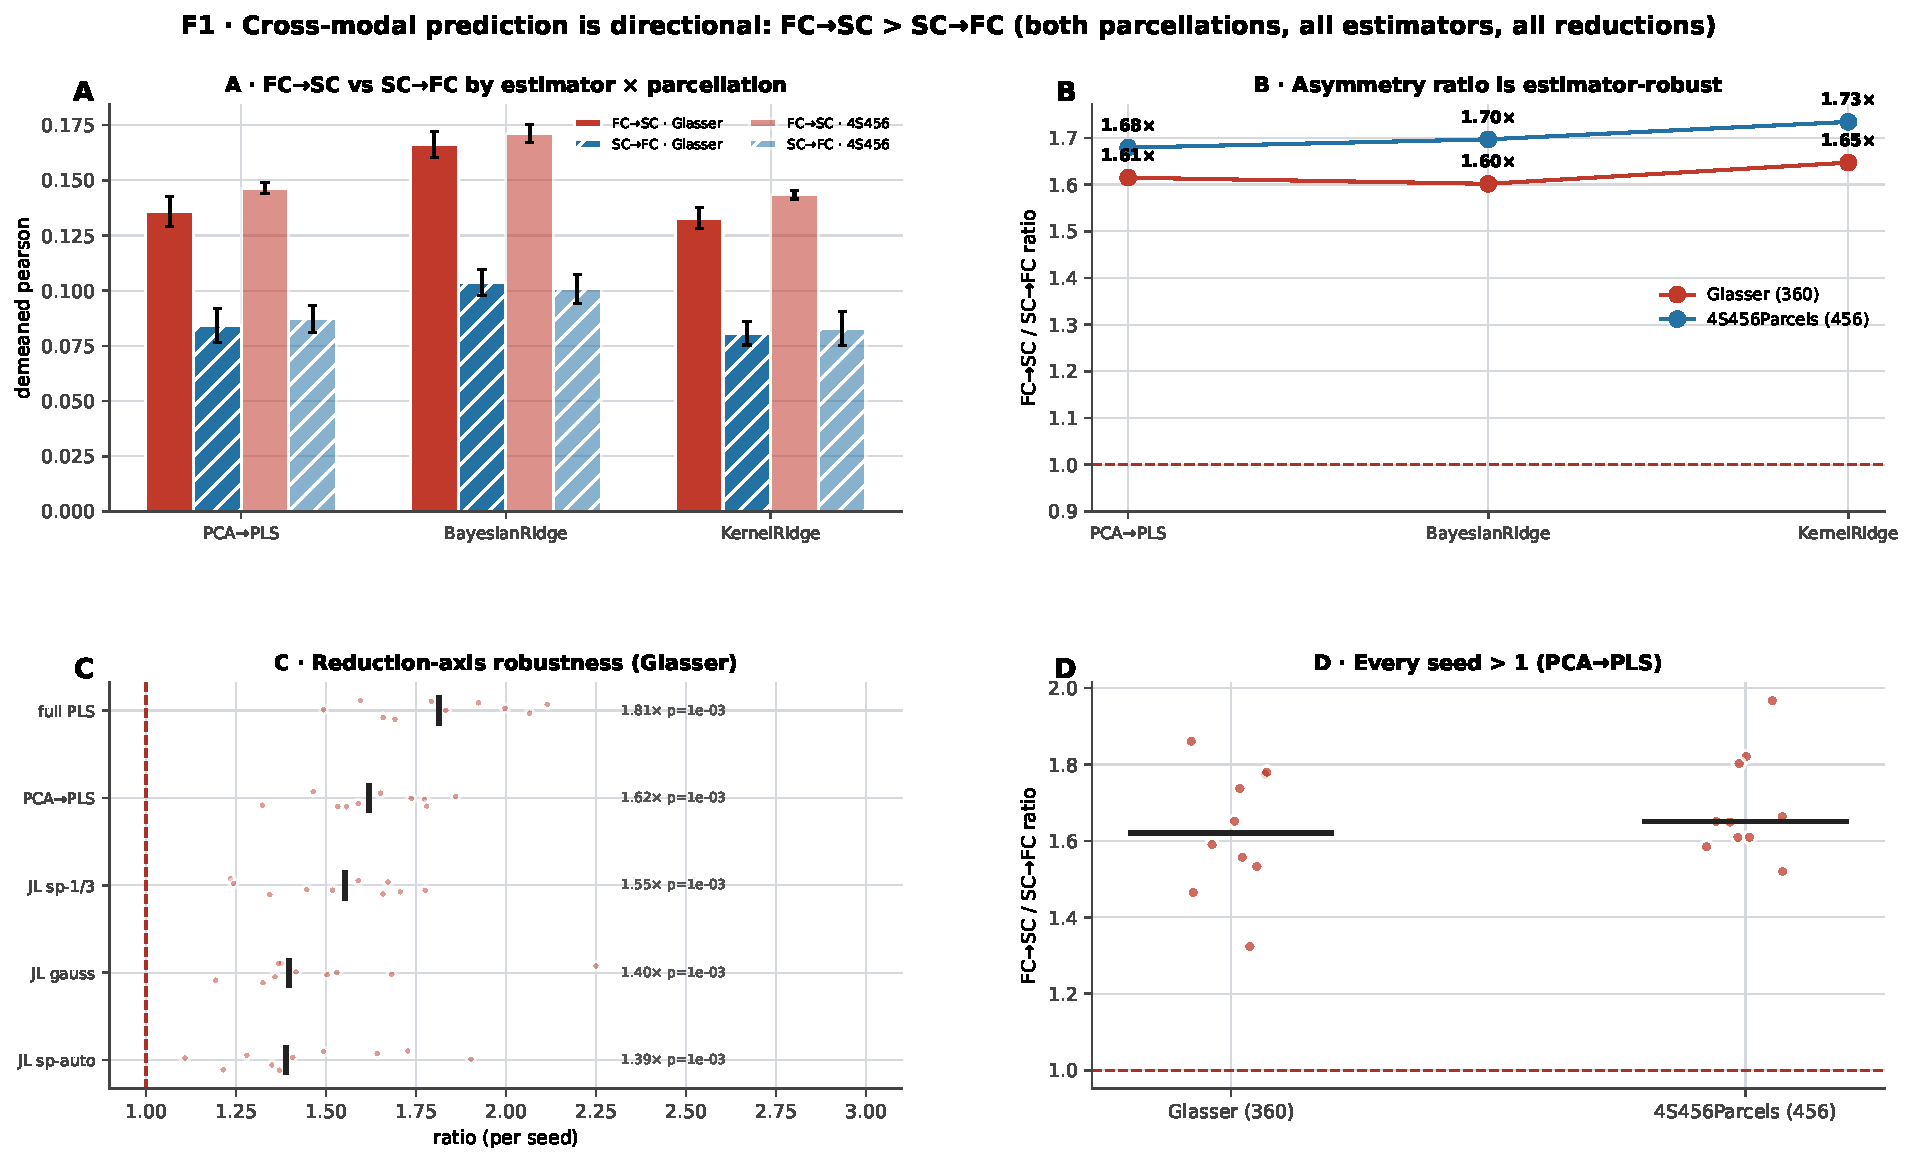
\includegraphics[width=\linewidth]{F1_directional_asymmetry.pdf}
\caption{\textbf{F1.} (A) \fcsc{} vs \scfc{} by estimator and parcellation; (B) the ratio is
estimator-robust; (C) and survives every reduction axis; (D) every seed exceeds 1.}
\label{fig:f1}\end{figure}

\FloatBarrier
\section{F2 · Anatomy$\rightarrow$SC / demographics$\rightarrow$FC double dissociation}
\textbf{Claim.} ``Subject information'' is not one generic confound: brain-volume features
predict SC better than demographics do, while demographics predict FC more than twice as well
as brain volumes do.

\textbf{Across parcellations (PCA$\rightarrow$PLS, \dpear).} Glasser: bv$\rightarrow$SC 0.162
$>$ demo$\rightarrow$SC 0.130, but demo$\rightarrow$FC 0.111 $>$ bv$\rightarrow$FC 0.049
(a $>2\times$ gap). The same crossover holds in 4S456 (Fig.~\ref{fig:f2}A--B).

\textbf{Across estimators.} The dissociation index (bv $-$ demo) is positive for
$\rightarrow$SC and negative for $\rightarrow$FC under all three estimators and both
parcellations (Fig.~\ref{fig:f2}C), so the crossover is not estimator-specific.

\textbf{Status.} \repl. \emph{Caveat (see needed-experiments E2):} brain volume mechanically
inflates streamline counts, so part of the bv$\rightarrow$SC arm may be a tractography
construction effect; a volume-normalized SC re-run is the clean test.

\begin{figure}[h]\centering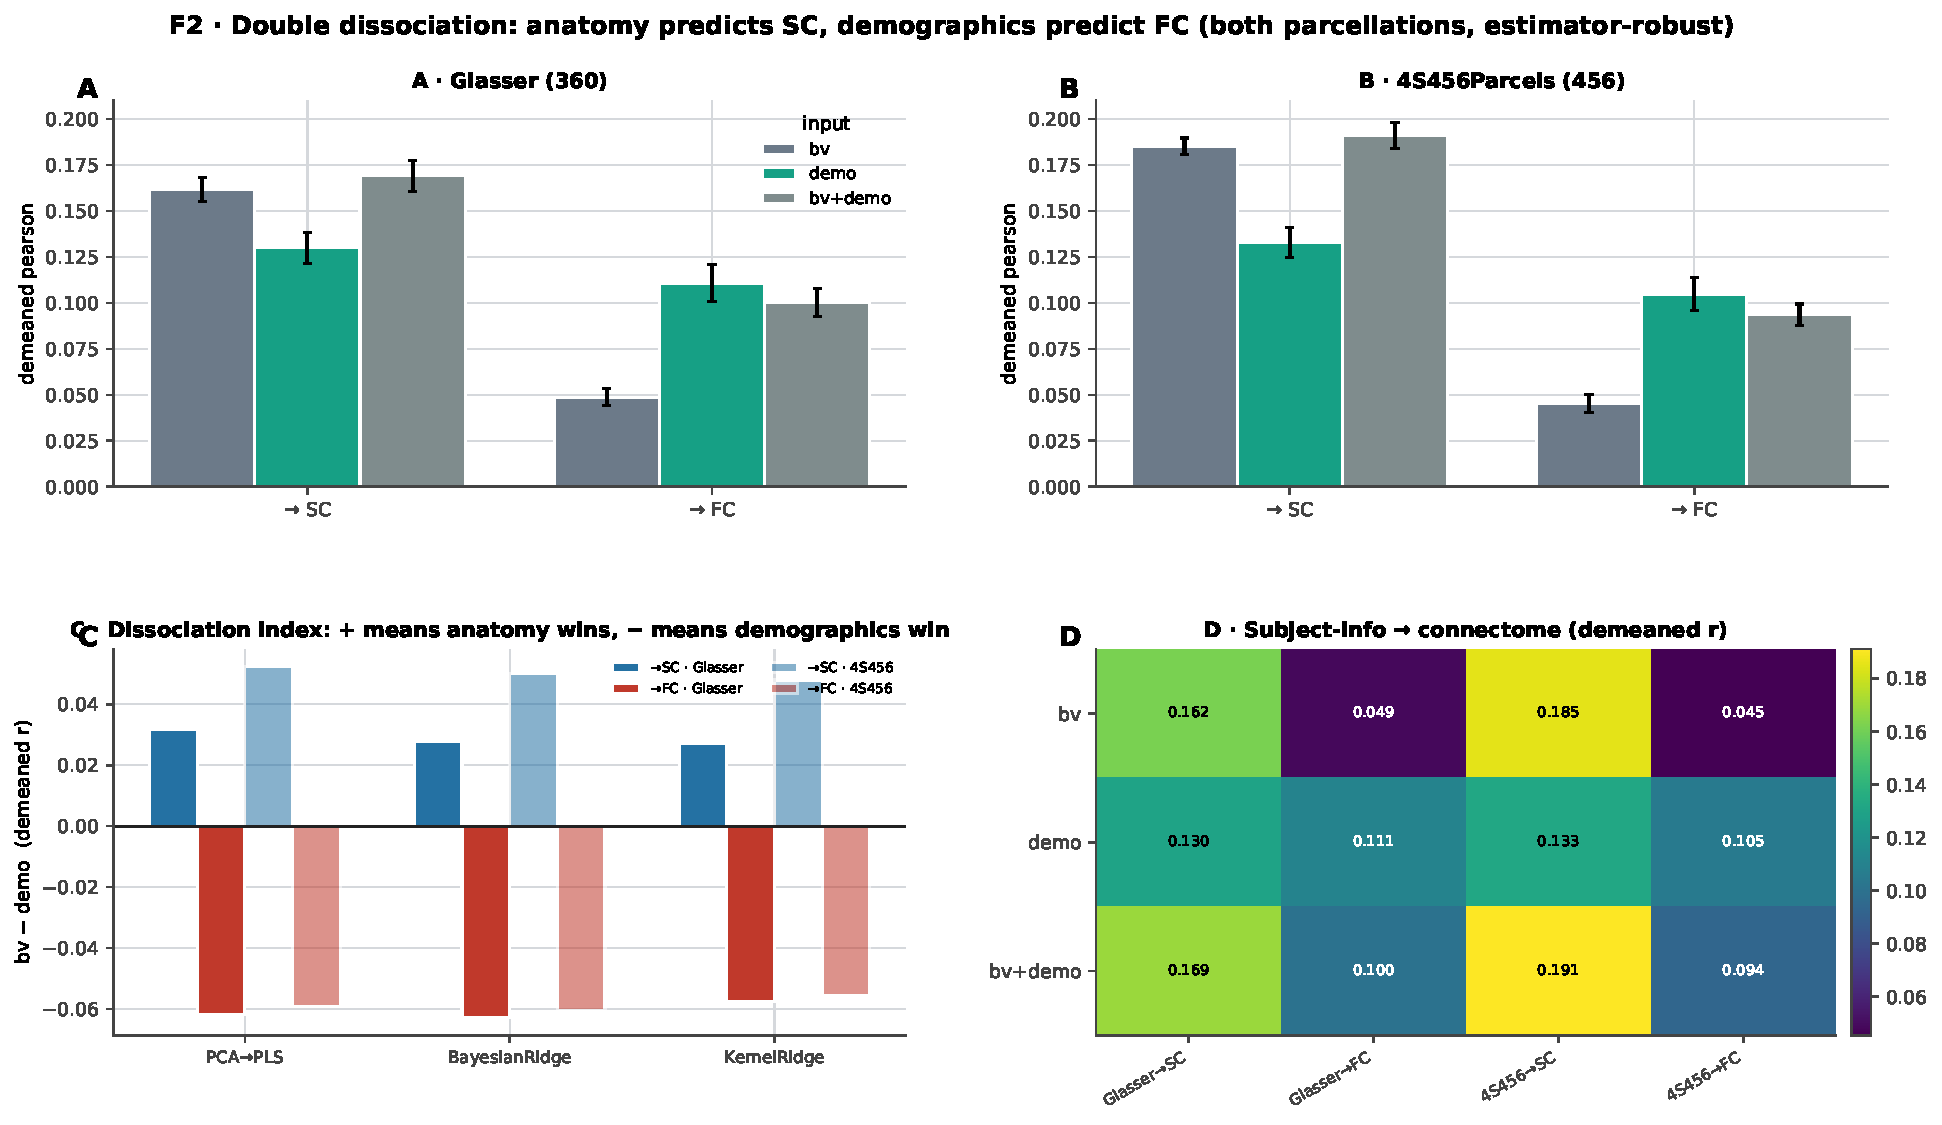
\includegraphics[width=\linewidth]{F2_double_dissociation.pdf}
\caption{\textbf{F2.} (A,B) subject-information inputs $\rightarrow$ SC and FC per parcellation;
(C) dissociation index across estimators; (D) full input$\times$target$\times$parcellation map.}
\label{fig:f2}\end{figure}

\FloatBarrier
\section{F3 · Imputed connectomes are measurable, but their utility is asymmetric}
\textbf{Claim.} Cross-modal prediction yields real, non-trivial imputed connectomes --- but
whether the imputed connectome is \emph{useful} depends on direction, and is interpreted
through F5.

\textbf{Across parcellations.} Both imputations are measurable: pred\_SC (from FC) reaches
\dpear{} 0.136/0.146 and pred\_FC (from SC) 0.084/0.087 (Fig.~\ref{fig:f3}A). Yet downstream
(Fig.~\ref{fig:f3}B--C) pred\_SC is roughly neutral on cognition while pred\_FC is harmful in
both atlases --- reconstruction quality and downstream utility are disconnected (a measurable
connectome is not necessarily a useful one).

\textbf{Status.} \repl, interpreted through F5.

\begin{figure}[h]\centering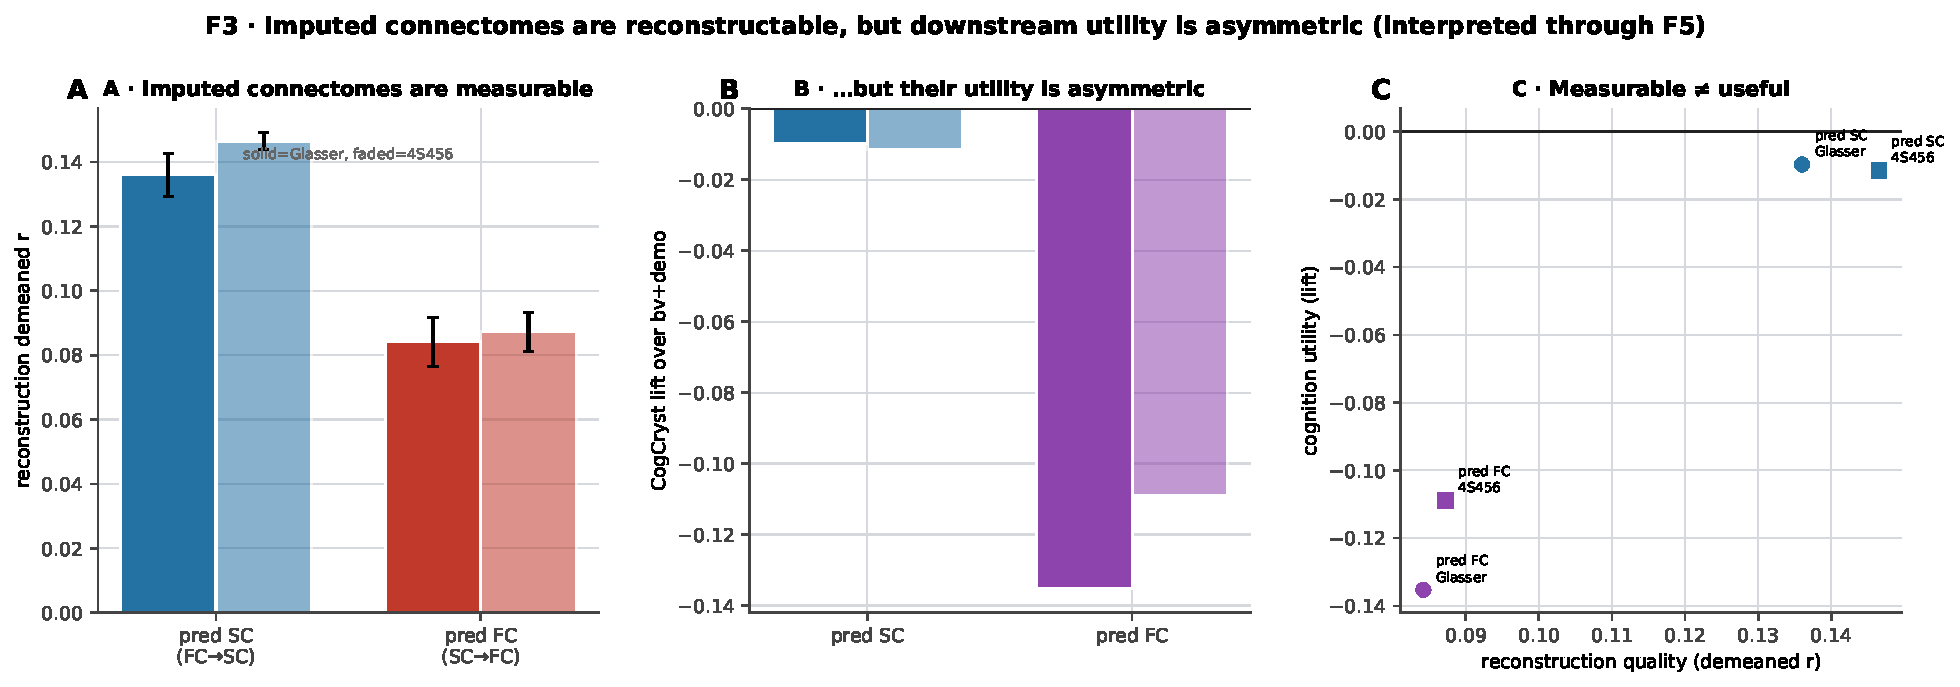
\includegraphics[width=\linewidth]{F3_imputation_usable_asymmetric.pdf}
\caption{\textbf{F3.} (A) imputed connectomes are reconstructable; (B) but their cognition
utility is asymmetric; (C) the measurable-vs-useful disconnect.}
\label{fig:f3}\end{figure}

\FloatBarrier
\section{F4 · Observed FC carries a crystallized-cognition signal (narrow, FDR-surviving)}
\textbf{Claim (stated at its defensible width, not walked back later).} Observed FC carries a
\emph{crystallized}-cognition signal that survives demographic residualization and
restricted-family multiplicity correction in the single cell obs FC$+$bv$+$demo
$\rightarrow$ CogCryst. The \emph{broader} ``FC beats the baseline on cognition'' framing is
real but multiplicity-fragile (see F11) and is \emph{not} the headline.

\textbf{The surviving cell (BayesianRidge).} obs FC$+$bv$+$demo $\rightarrow$ CogCryst lifts
$+0.162$ (Glasser) / $+0.146$ (4S456) over \bvdemo, survives restricted-family FDR
($q=0.027$ / $0.048$, F11), and survives residualization on \bvdemo{} (Fig.~\ref{fig:f4}B).
Plain obs FC $\rightarrow$ CogCryst (lifts $+0.133$ / $+0.122$) is nominal-only (whole-grid
$q\approx0.24$). CogTotal lifts are smaller ($+0.088$/$+0.086$) and CogFluid smaller again ---
the effect is carried specifically by crystallized cognition.

\textbf{Across estimators.} The lift is positive under PCA$\rightarrow$PLS and BayesianRidge;
KernelRidge scalar rows are shown only to expose the instability described in the estimator note
(Fig.~\ref{fig:f4}C). BayesianRidge is the reportable estimator.

\textbf{Status.} \repl{} for the narrow cell; the broad cognition claim is multiplicity-fragile
(F11). This narrow framing is consistent with F11 by construction --- F4 and F11 state the same
corrected claim, not a strong claim and a later retraction.

\begin{figure}[h]\centering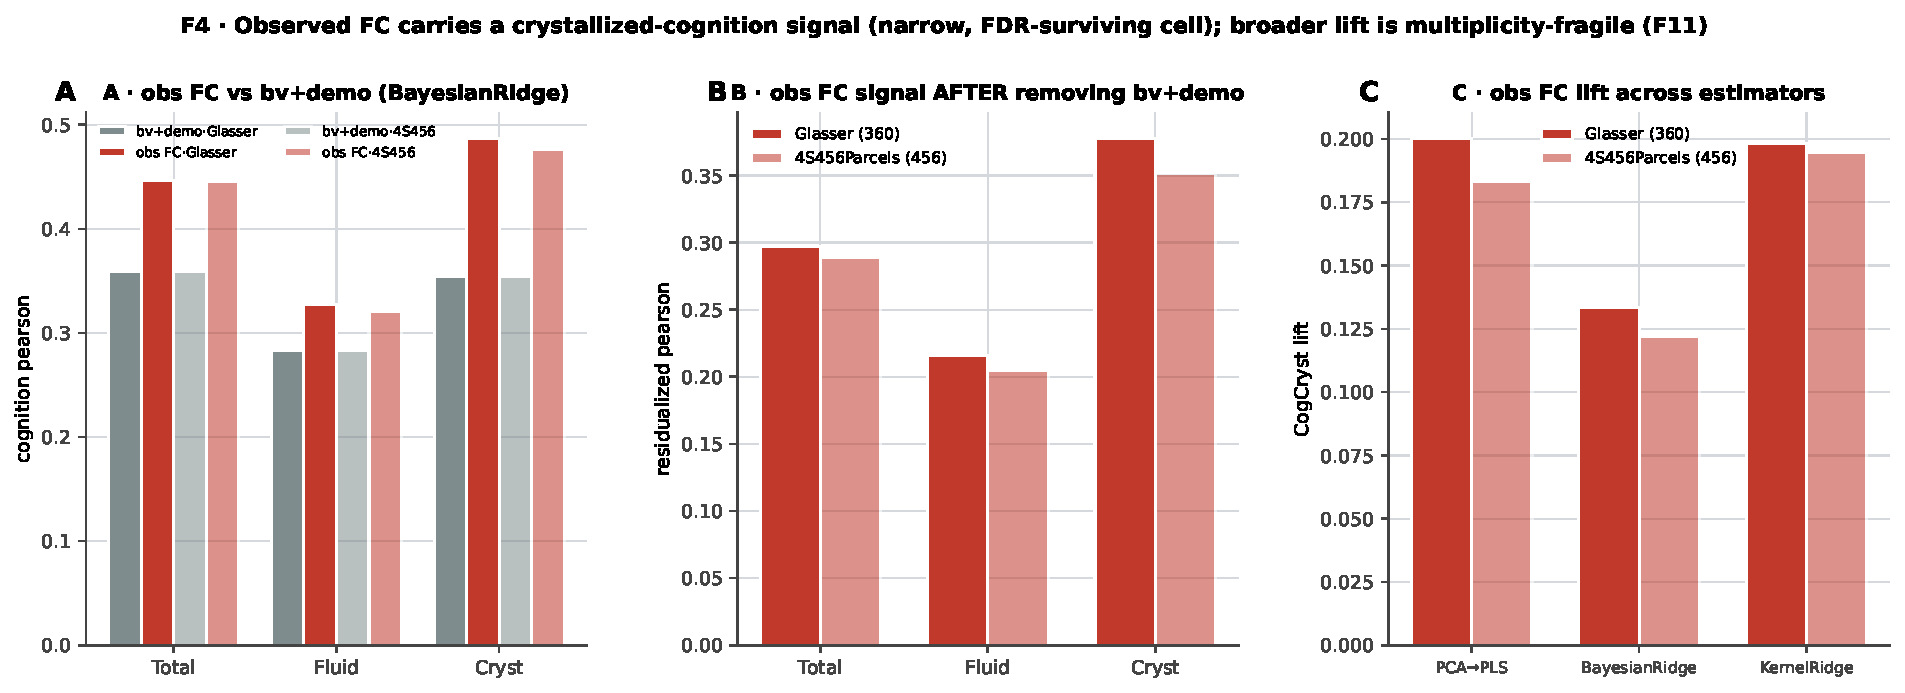
\includegraphics[width=\linewidth]{F4_obs_fc_cognition.pdf}
\caption{\textbf{F4.} (A) obs FC vs \bvdemo{} for three cognitive targets; (B) FC signal after
removing \bvdemo; (C) obs FC CogCryst lift across estimators.}
\label{fig:f4}\end{figure}

\FloatBarrier
\section{F5 · SC underperforms, imputation does not transfer utility, pred\_FC is harmful}
\textbf{Claim.} Observed SC does not clear \bvdemo{} for cognition, imputed connectomes do not
transfer FC's utility, and FC imputed from SC is actively below baseline.

\textbf{Across parcellations (BayesianRidge lift over \bvdemo).} Observed SC is below baseline
on all three targets in both atlases (e.g.\ CogCryst $-0.101$ / $-0.095$). pred\_FC is
consistently the most harmful (CogCryst $-0.135$ / $-0.109$), while pred\_SC is roughly neutral
to slightly negative (Fig.~\ref{fig:f5}A--B,D). The contrast pred\_SC vs pred\_FC at matched
dimensionality shows the harm is direction-specific.

\textbf{Across estimators.} Under BayesianRidge (reportable) and PCA$\rightarrow$PLS the
negatives hold; the KernelRidge scalar bars flip sign (Fig.~\ref{fig:f5}C) --- the instability
of the estimator note, not evidence SC helps.

\textbf{Status.} \repl.

\begin{figure}[h]\centering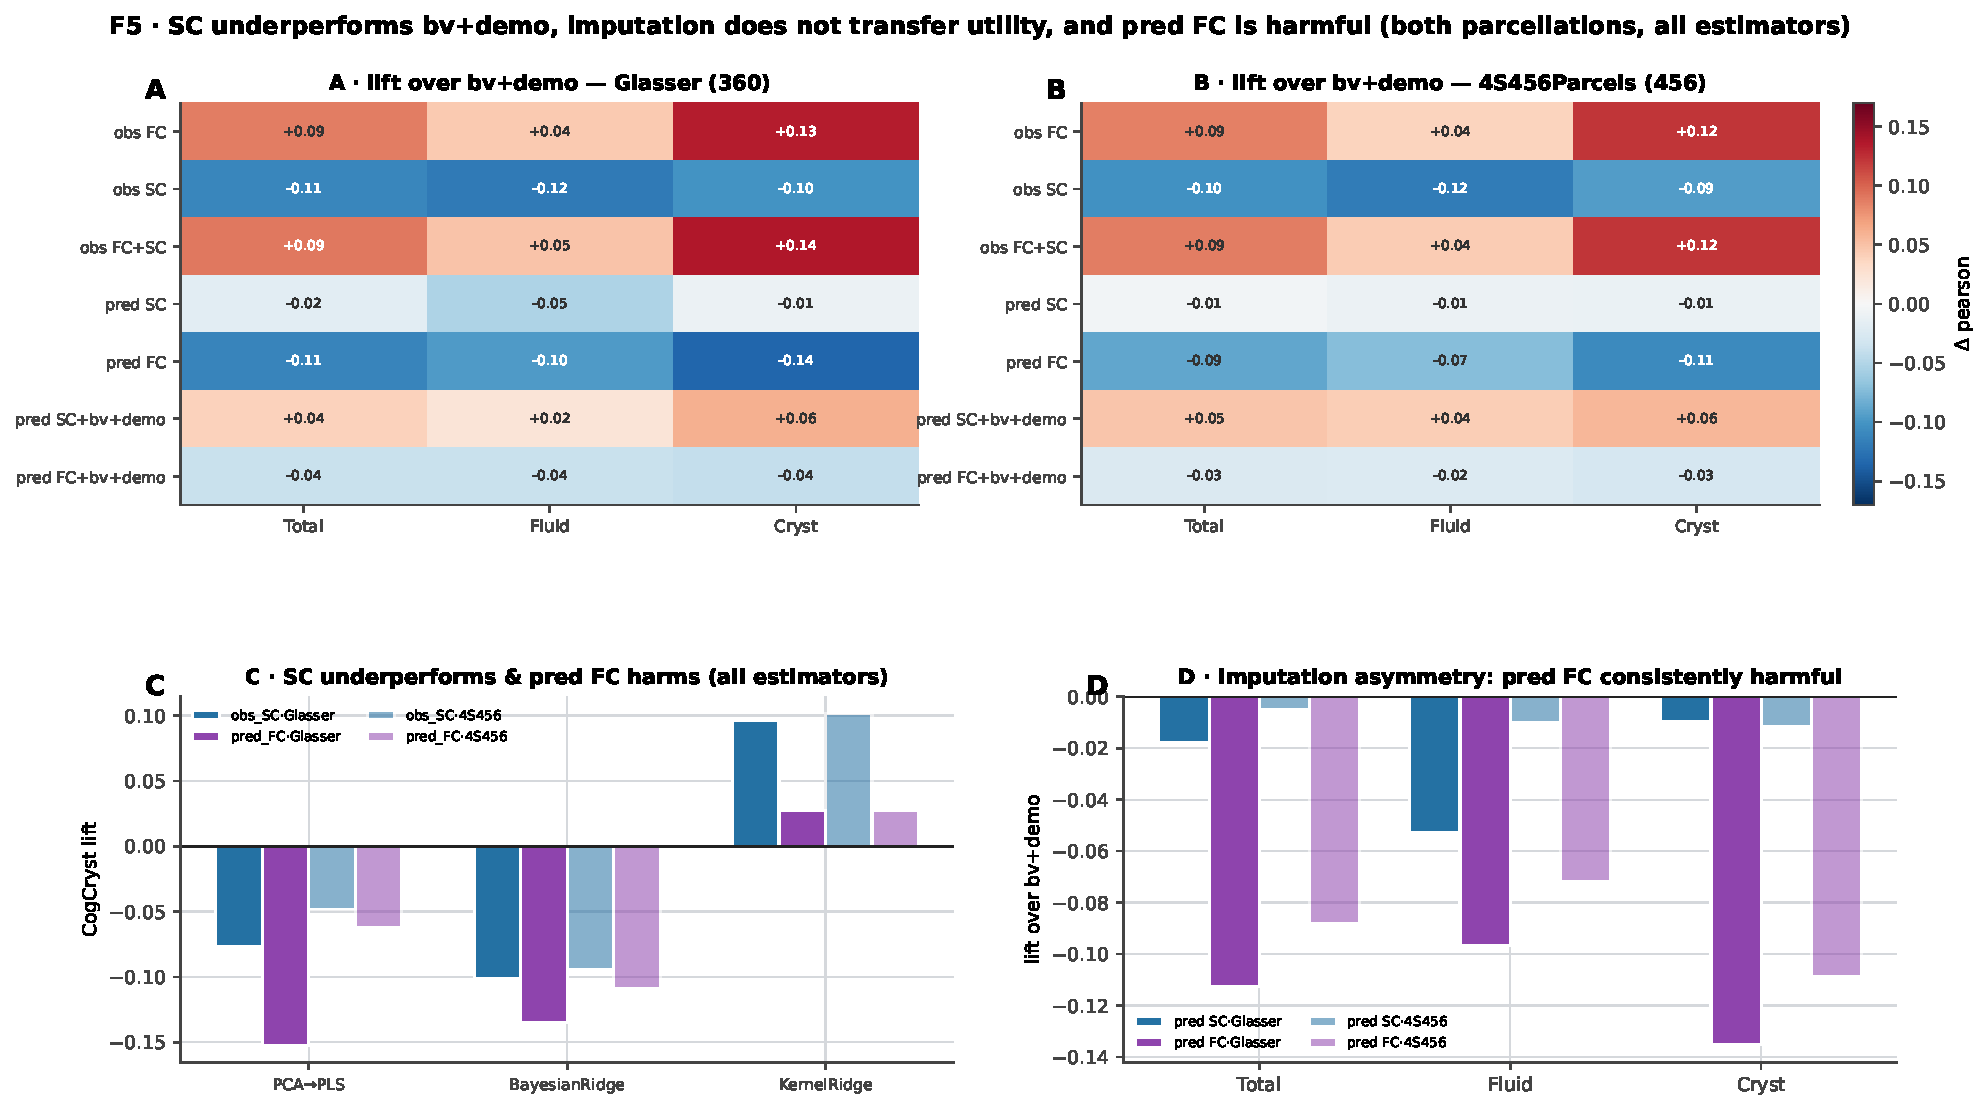
\includegraphics[width=\linewidth]{F5_utility_wall.pdf}
\caption{\textbf{F5.} (A,B) full lift-over-\bvdemo{} maps per parcellation; (C) SC/pred\_FC
harm across estimators (note KR instability); (D) pred\_FC harm is consistent across targets.}
\label{fig:f5}\end{figure}

\FloatBarrier
\section{F6 · Predicted connectomes carry heritable family signal}
\textbf{Claim.} SC predicted from FC preserves individualized, heritable structure not reducible
to \bvdemo.

\textbf{Across parcellations.} Residualized predicted SC separates siblings at AUC $\approx
0.81$ (Glasser) / $0.82$ (4S456), far above the \bvdemo{} baseline ($\approx 0.56$); the signal
strengthens monotonically from siblings to DZ to MZ twins (Fig.~\ref{fig:f6}). The
sibling-AUC gain over baseline is $\approx +0.25$ in both atlases.

\textbf{Source.} F6--F8 come from the separate family-mechanism pipeline
(\texttt{reproduction/family\_mechanism/outputs/}), which adds the sibling/twin task on top of
the same frozen family-aware splits; this task is not part of the three main grid CSVs.

\textbf{Status.} \repl{} (family-mechanism pipeline, both parcellations).

\begin{figure}[h]\centering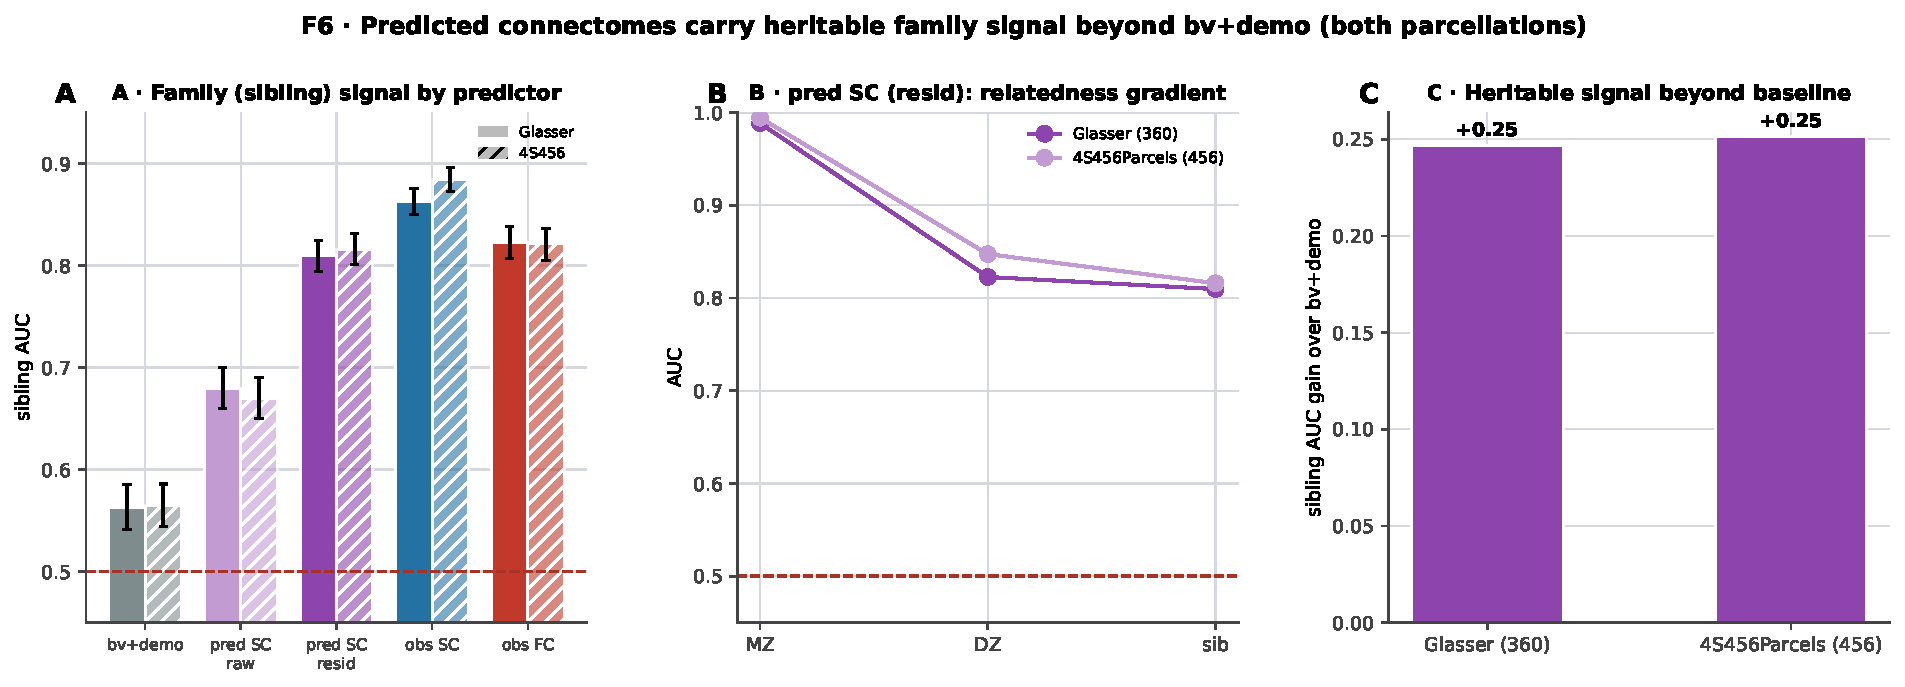
\includegraphics[width=\linewidth]{F6_family_signal.pdf}
\caption{\textbf{F6.} (A) sibling AUC by predictor; (B) MZ/DZ/sibling gradient for residualized
predicted SC; (C) AUC gain over the \bvdemo{} baseline.}
\label{fig:f6}\end{figure}

\FloatBarrier
\section{F7 · Reconstruction and identification objectives trade off}
\textbf{Claim.} A predictor optimized for reconstruction does not preserve identity signal: the
same imputed-SC pipeline can carry family signal or lose it depending on the objective.

\textbf{Across parcellations.} The reconstruction-optimized ``combined'' predictor keeps strong
MZ/DZ separation but collapses to chance ($\approx 0.50$) for siblings in both atlases, whereas
the residualized predictor retains sibling signal ($\approx 0.81$) (Fig.~\ref{fig:f7}). One
predicted connectome cannot serve every objective.

\textbf{Status.} \repl.

\begin{figure}[h]\centering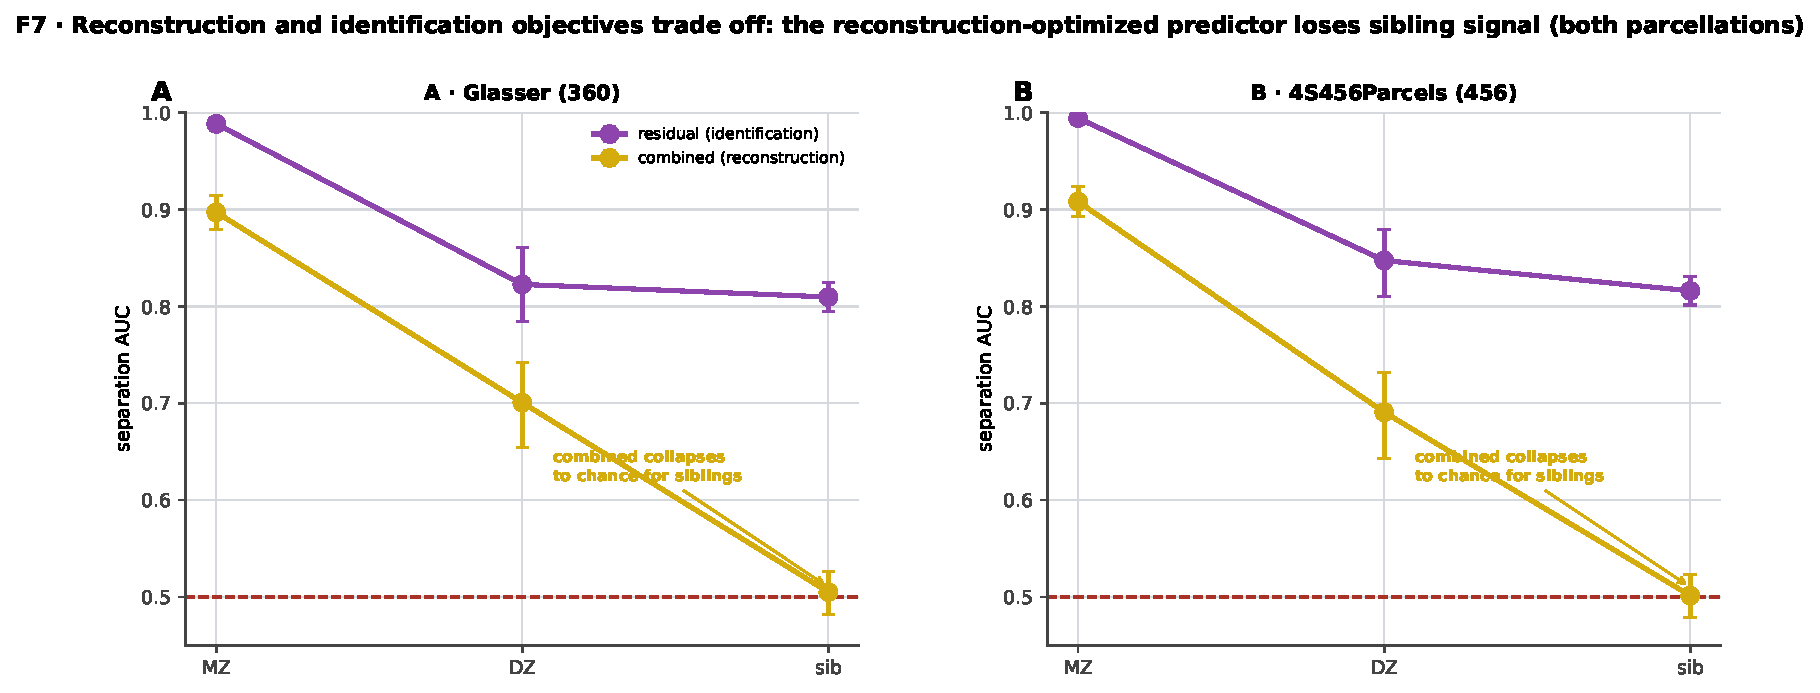
\includegraphics[width=\linewidth]{F7_objective_tradeoff.pdf}
\caption{\textbf{F7.} Residual (identification) vs combined (reconstruction) predictors across
relatedness, per parcellation; the combined predictor collapses for siblings.}
\label{fig:f7}\end{figure}

\FloatBarrier
\section{F8 · Exploratory mechanism: an FC-predictable low-variance SC mode (component index not stable)}
\textbf{Claim (the claim is a \emph{property}, not a component identity).} Part of the family
signal localizes to a small, FC-predictable, low-variance, family-discriminative, low-confound,
visual/dorsal-attention-localized SC mode. \textbf{The component \emph{index} is not a
meaningful quantity} --- the mode that carries this property is the 3rd PC under Glasser and the
4th under 4S456, and this migration is exactly why we make no claim about a numbered component;
only the property is the finding. ``PC3/PC4'' below are pointers to where the property landed in
each atlas, not an identity to track.

\textbf{Across parcellations.} The property-bearing mode (Glasser 3rd, 4S456 4th;
Fig.~\ref{fig:f8}A) has, among the non-PC1 components, the highest FC$\rightarrow$PC
predictability ($R^2\approx 0.22$/$0.24$), sibling AUC $\approx 0.58$, and near-zero sex/volume
confound. \textbf{PC1 is a confound} ($R^2\approx 0.89$--$0.93$ with sex/volume;
Fig.~\ref{fig:f8}B) and is not a mechanism. The mode is cross-seed stable (Fig.~\ref{fig:f8}C)
and localizes to visual / dorsal-attention edges (Fig.~\ref{fig:f8}D), a localization that
survives strength+distance+reliability partialling (41\% of $|$mode$|$).

\textbf{Status.} \partialst. The property replicates across atlases; the component \emph{label}
does not, and is not claimed.

\begin{figure}[h]\centering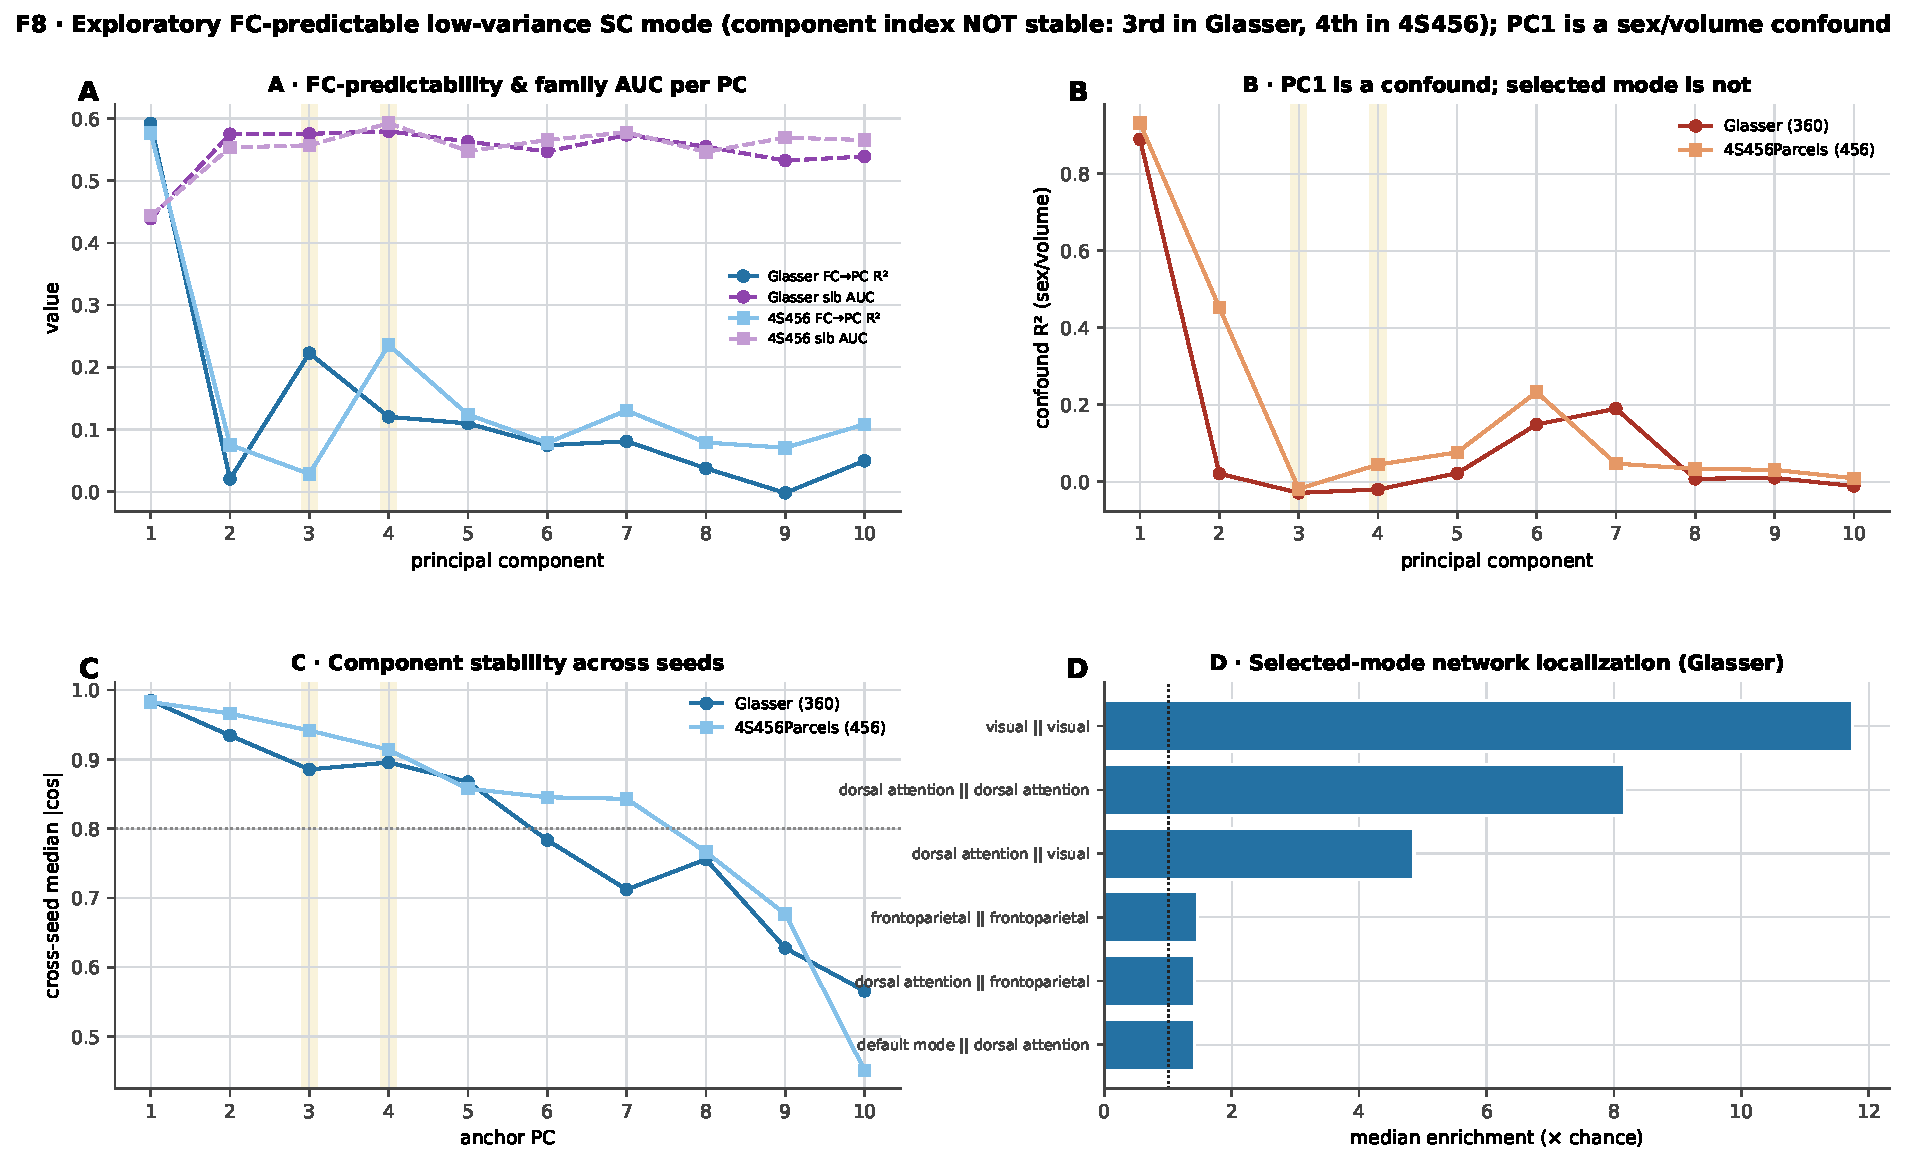
\includegraphics[width=\linewidth]{F8_pc_mechanism.pdf}
\caption{\textbf{F8.} (A) FC-predictability and sibling AUC per PC; (B) PC1 confound; (C)
cross-seed stability; (D) network localization of the selected mode.}
\label{fig:f8}\end{figure}

\FloatBarrier
\section{F9 · Richer tractography does not help}
\textbf{Claim.} Named-bundle tractography (\texttt{r2t}) does not recover the missing structural
signal that streamline counts miss.

\textbf{Evidence (Glasser, exploratory).} \texttt{r2t} predicts FC \emph{worse} than count-SC
(\dpear{} 0.049 vs 0.085), adds nothing marginal over counts ($\Delta=-0.001$), and carries no
cognition signal above \bvdemo{} --- every tractography representation, including the
\texttt{r2t}$\rightarrow$synthetic-FC substitution chain, falls below the floor
(Fig.~\ref{fig:f9}). The \fcsc{} asymmetry holds across representations. Counts are a sufficient
statistic for cross-modal prediction.

\textbf{Status.} Glasser / exploratory (the r2t bundle features were derived for Glasser).

\begin{figure}[h]\centering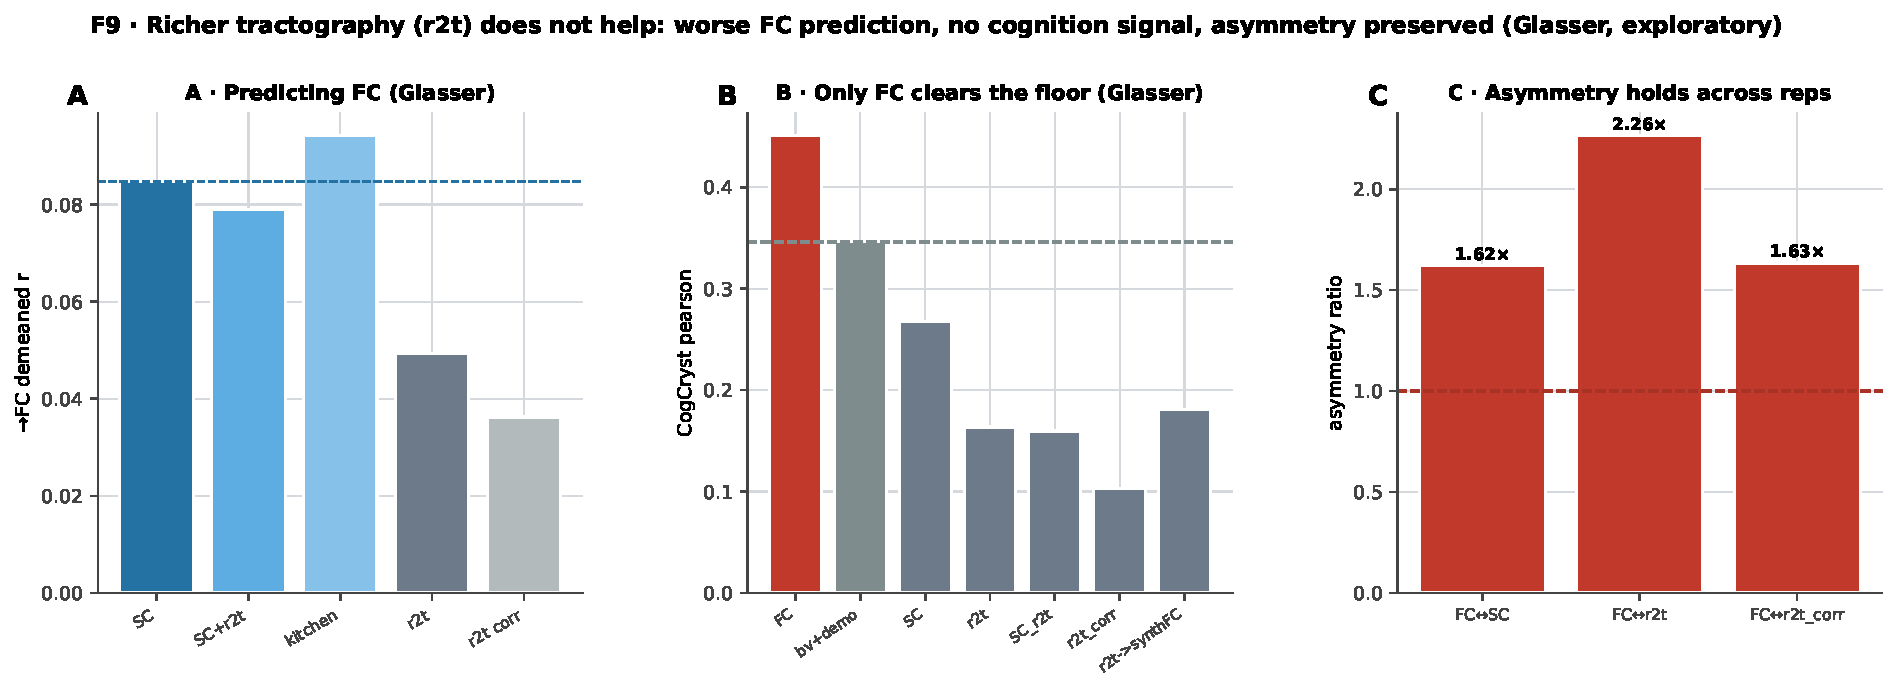
\includegraphics[width=\linewidth]{F9_tractography.pdf}
\caption{\textbf{F9.} (A) predicting FC from each structural representation; (B) downstream
cognition by representation; (C) the asymmetry is preserved across representations.}
\label{fig:f9}\end{figure}

\FloatBarrier
\section{F10 · Nonlinear models and more data do not break the ceiling}
\textbf{Claim.} The linear ceiling is structural in this regime, not a model-capacity or
sample-size artifact, and the \scfc{} shortfall is not FC measurement noise.

\textbf{Evidence.} The nonlinear$-$linear gap stays $\le 0$ from $n=100$ to $n\approx 683$ while
the linear score climbs (Fig.~\ref{fig:f10}A--B); the KernelRidge 9-variant hyperparameter
sweep is nearly degenerate (within-seed spread $\approx 0.004$--$0.005$;
Fig.~\ref{fig:f10}C); and \scfc{} reaches only $\sim$17\% of the FC between-session reliability
ceiling, with per-subject achieved quality uncorrelated with FC reliability
(Fig.~\ref{fig:f10}D). The reliability accounting is computed in both parcellations; the
scaling/nonlinear probes are Glasser.

\textbf{Status.} Glasser / exploratory for the nonlinear+scaling probes; the reliability
ceiling replicates in both parcellations.

\begin{figure}[h]\centering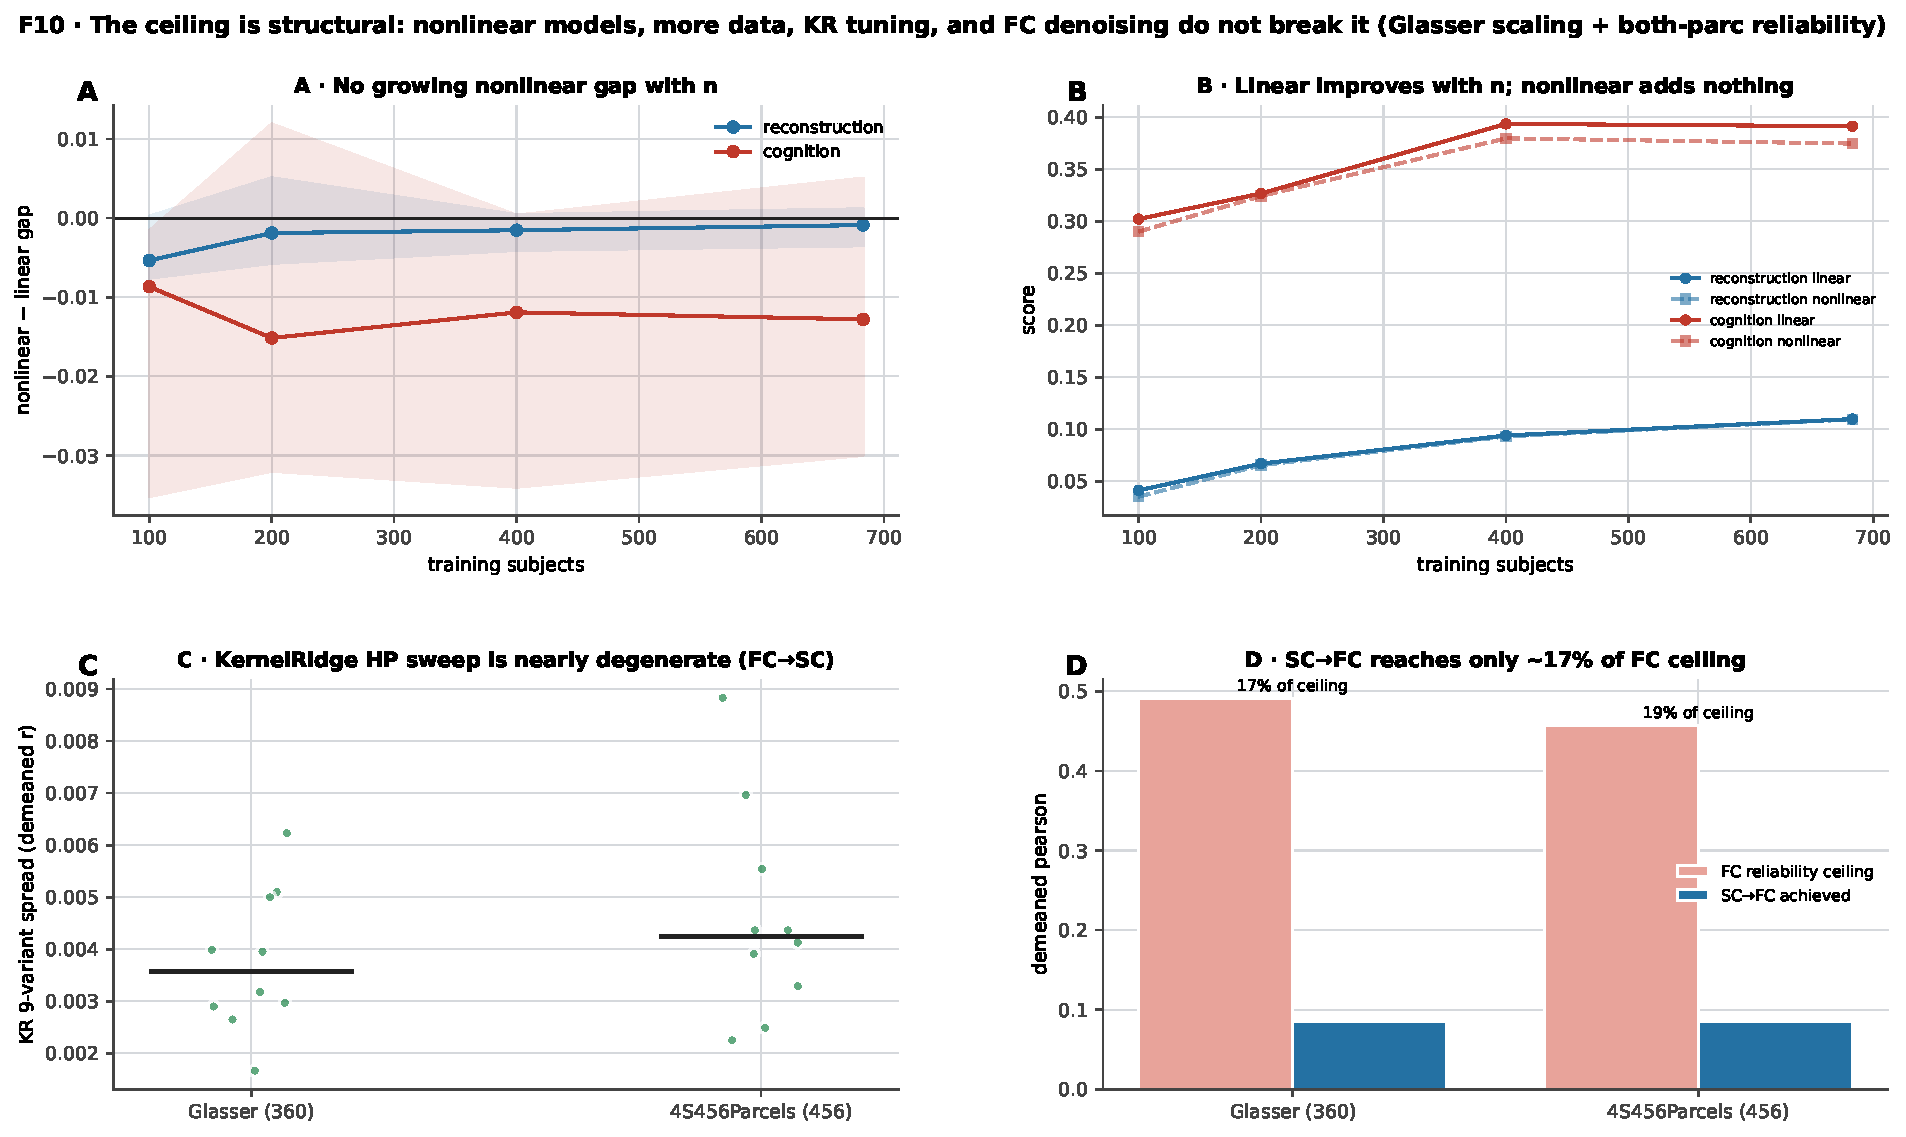
\includegraphics[width=\linewidth]{F10_structural_ceiling.pdf}
\caption{\textbf{F10.} (A) nonlinear gap vs $n$; (B) linear improves with $n$, nonlinear does
not; (C) KernelRidge HP flatness; (D) \scfc{} vs the FC reliability ceiling in both atlases.}
\label{fig:f10}\end{figure}

\FloatBarrier
\section{F11 · The observed-FC cognition lift is real but multiplicity-fragile}
\textbf{Origin.} This finding is from the robustness analysis added in this work (not in the
original F1--F10 ledger). It stress-tests F4.

\textbf{Claim.} Observed FC's cognition lift over \bvdemo{} is genuine but sits close to the
edge of significance once multiplicity and uncertainty are handled honestly.

\textbf{Evidence (both parcellations, BayesianRidge).} With 95\% seed CIs and BH-FDR over the
downstream grid: \emph{zero} positive lifts survive whole-grid FDR (54 cells); under a
restricted affirmative family (observed-FC cognition, 12 cells) only obs FC$+$bv$+$demo
$\rightarrow$ CogCryst survives (family $q=0.027$ Glasser / $0.048$ 4S456), while plain obs FC
$\rightarrow$ CogCryst is nominal only (uncorrected $p\approx0.03$--$0.04$, whole-grid
$q\approx0.24$). The median minimum-detectable-effect at 80\% power is $\approx 0.056$ pearson:
the design is well-powered for the $\sim$0.1 lifts of interest, underpowered below $\sim$0.03
(Fig.~\ref{fig:f11}).

\textbf{Status.} Both parcellations (this analysis). The affirmative claim should be reported as
restricted-family-corrected with CIs, not as a bare $p<0.05$.

\begin{figure}[h]\centering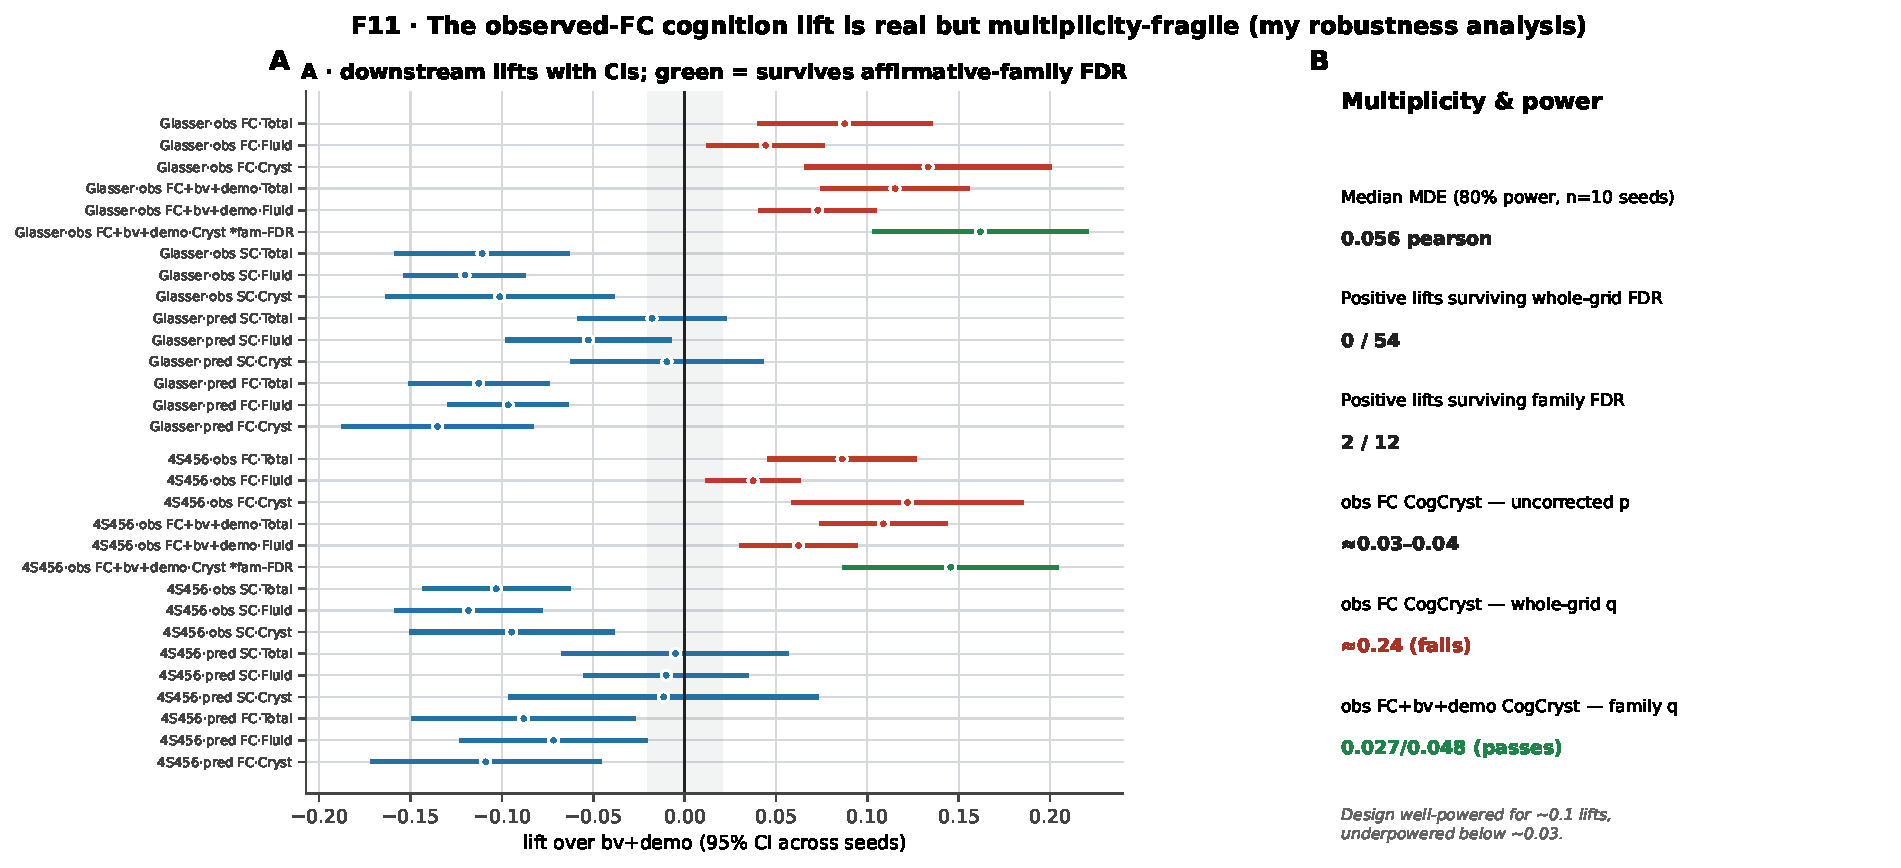
\includegraphics[width=\linewidth]{F11_statistical_fragility.pdf}
\caption{\textbf{F11.} (A) downstream lifts with 95\% CIs; green = survives affirmative-family
FDR. (B) multiplicity and power summary.}
\label{fig:f11}\end{figure}

\FloatBarrier
\section{F12 · Bayesian corroboration (shrinkage, ROPE, Bayes factors)}
\textbf{Origin.} A Bayesian re-analysis added in this work, corroborating F4/F5/F11 under a
different inferential framework.

\textbf{Claim.} The frequentist conclusions hold as posterior statements: the negatives are
credibly at/below a practical-equivalence region, and the positive lift is supported only for
the strongest cells.

\textbf{Evidence.} A hierarchical partial-pooling model (PyMC NUTS) over the affirmative family
shrinks each cell toward the family mean (grand-mean lift $\approx +0.10$); 11/12 cells keep a
95\% HDI above the ROPE ($\pm0.02$), with obs FC$+$bv$+$demo $\rightarrow$ CogCryst the most
robust. JZS Bayes factors show strong evidence of a \emph{harmful} effect for observed SC and
pred\_FC (not a null), and P(pred\_FC lift $<0)\approx1$ (Fig.~\ref{fig:f12}).

\textbf{Caveat.} These posteriors use the 10 seed-level lifts, so they are the Bayesian
counterpart of the seed-level test (which excluded zero), not of the subject-level permutation
test; because seeds are pseudo-replicated resplits, the Bayes-factor magnitudes overstate the
evidence and should be read with that unit-of-analysis caveat.

\textbf{Status.} Both parcellations (this analysis).

\begin{figure}[h]\centering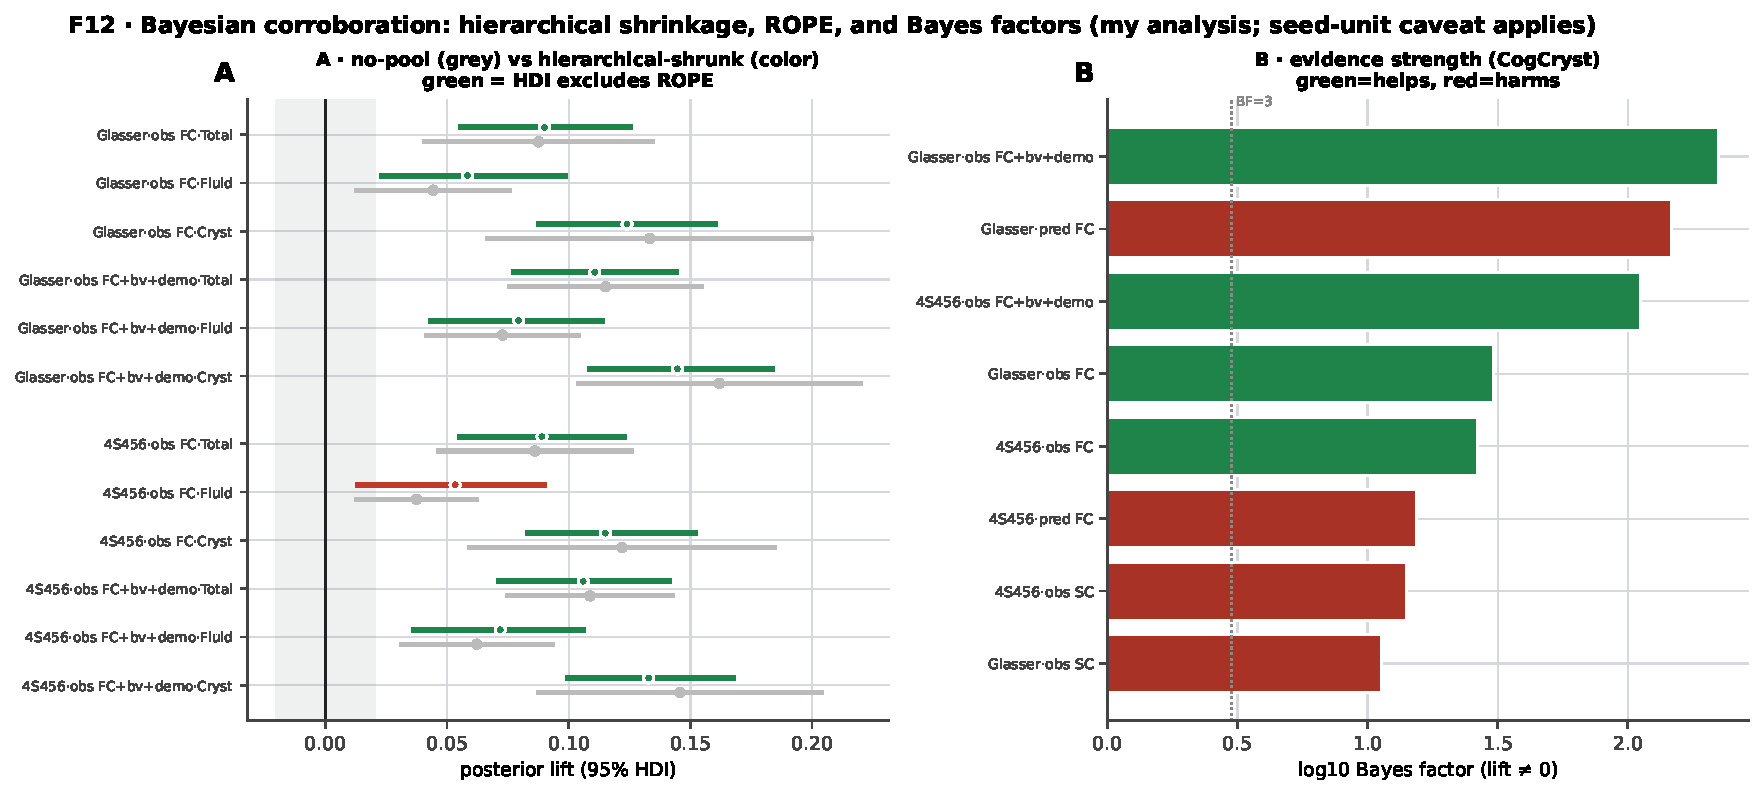
\includegraphics[width=\linewidth]{F12_bayesian_corroboration.pdf}
\caption{\textbf{F12.} (A) no-pooling vs hierarchical-shrunk posterior HDIs against the ROPE;
(B) Bayes factors coloured by effect direction (green helps, red harms).}
\label{fig:f12}\end{figure}

\FloatBarrier
\section{F13 · Imputation harm is direction-specific; cross-modal loss vs the oracle}
\textbf{Origin.} Two quantitative results from this analysis that sharpen F3/F5 and F1/F10.

\textbf{Claim 1 — direction-specific harm.} pred\_FC's sub-baseline harm is not a generic
high-dimensional-input artifact: at matched dimensionality, pred\_FC is $\sim$2--3$\times$ more
harmful than pred\_SC under BayesianRidge and PCA$\rightarrow$PLS in both parcellations
(Fig.~\ref{fig:f13}A). (KernelRidge scalar bars flip sign --- the instability of the estimator
note, shown for transparency, not interpreted.)

\textbf{Claim 2 — cross-modal loss.} Using a consistent same-estimator oracle
(PCA$\rightarrow$PLS), cross-modal prediction reaches only $\approx 19$--$21\%$ (\scfc{} / the
\mbox{FC$\rightarrow$FC} ceiling) and $\approx 36$--$38\%$ (\fcsc{} / the \mbox{SC$\rightarrow$SC}
ceiling) of the within-modality model ceiling, with credible intervals well below 1
(Fig.~\ref{fig:f13}B) --- the cross-modal loss is large and estimator-independent.

\textbf{Status.} Both parcellations (this analysis). The definitive imputation control
(spectrum-matched / group-mean surrogate) needs the imputation \texttt{.npy} artifacts and is
listed as a needed experiment.

\begin{figure}[h]\centering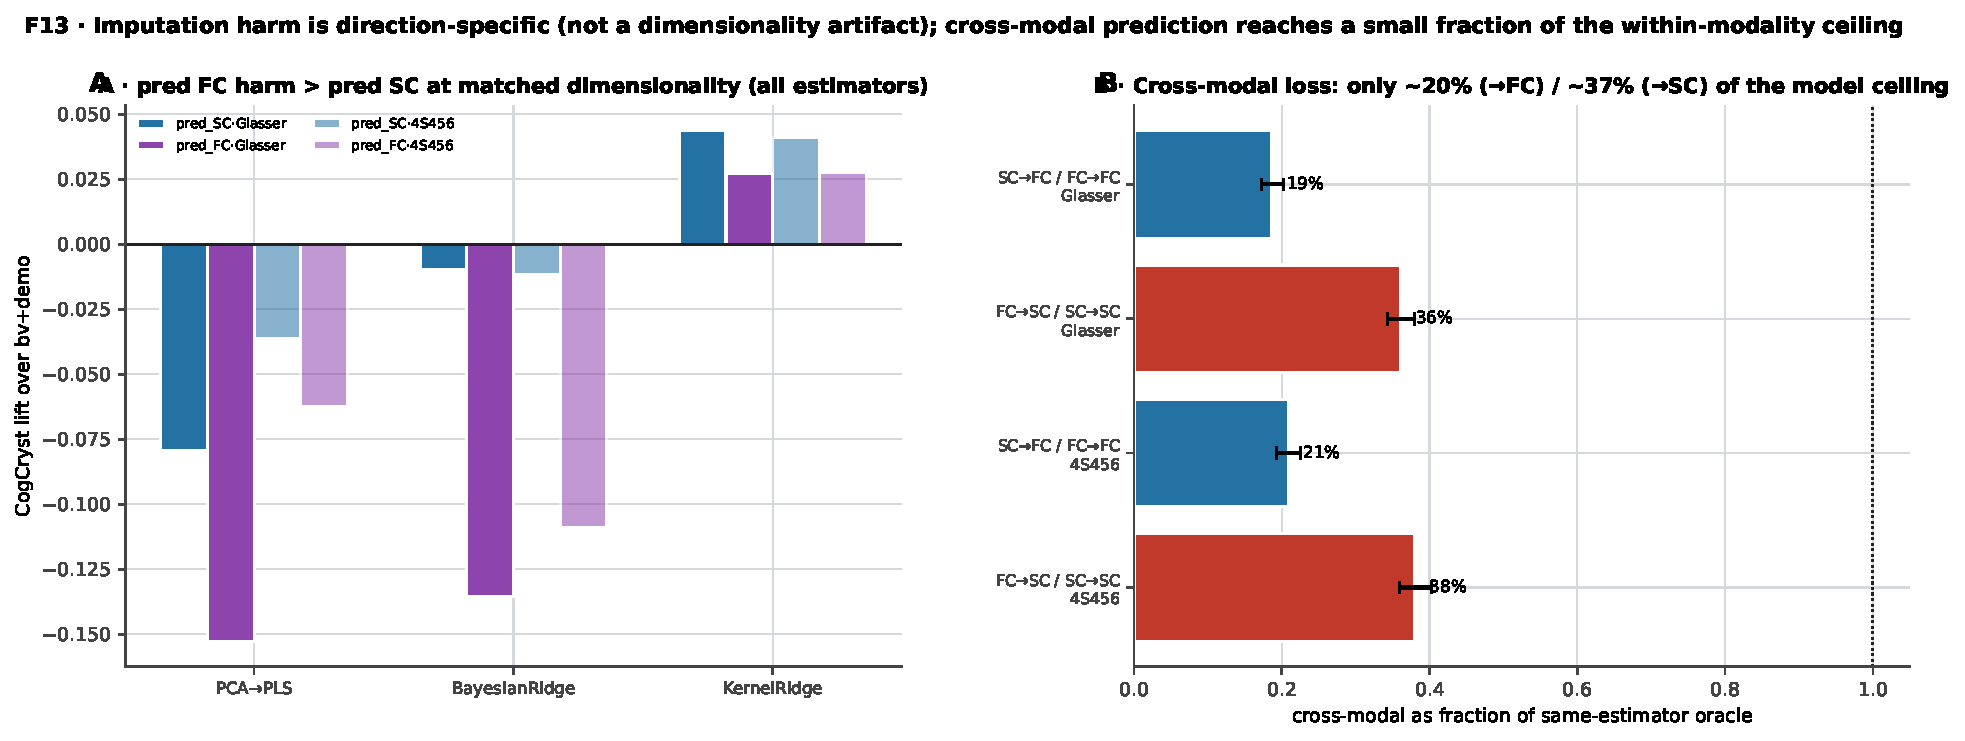
\includegraphics[width=\linewidth]{F13_imputation_and_oracle.pdf}
\caption{\textbf{F13.} (A) pred\_FC vs pred\_SC at matched dimensionality across estimators;
(B) cross-modal prediction as a fraction of the same-estimator within-modality oracle.}
\label{fig:f13}\end{figure}

\FloatBarrier
\section*{Synthesis}
Reading the ledger top to bottom: cross-modal prediction is \emph{directional} (F1) and the
subject-information confounds are \emph{structured} (F2); imputed connectomes are real but their
usefulness is \emph{direction-dependent} (F3), because only observed FC carries cognition signal
(F4) while SC and imputed connectomes do not clear the cheap baseline and pred\_FC is harmful
(F5). The constructive exception is identity: predicted connectomes carry heritable family
signal (F6), but only under objectives that preserve it (F7), and the mechanism is an
exploratory FC-predictable low-variance SC mode (F8). The negative results are not artifacts of
representation (F9) or of model class / sample size / FC noise (F10). Across all ten, the two
parcellations agree on every replicated finding; the estimator only matters for the
\emph{scalar} downstream KernelRidge rows, excluded on the principled grounds set out in the
estimator note.

Three further findings from this analysis tighten the picture: the one affirmative claim (F4)
is real but multiplicity-fragile (F11), and the same conclusion holds under a Bayesian
framework (F12); the imputation harm is direction-specific rather than a dimensionality
artifact, and cross-modal prediction reaches only a small fraction of the within-modality
oracle (F13).

\end{document}
